\documentclass[12pt,a4paper]{article}

%%%%%%%%%%%%%%%%%%%%%%%%%%%%%%%%%%%%%%%%
%%% Useful packages                  %%%
%%%%%%%%%%%%%%%%%%%%%%%%%%%%%%%%%%%%%%%%
% Authors should add any additional ones here             
\usepackage{lipsum} % For example text
\usepackage{amsmath}
\usepackage{graphicx}
\usepackage[numbers,sort&compress]{natbib} % adding the 'numbers' option provides numerical citations.
\usepackage[subtle]{savetrees} % condenses the text and reduces whitespace. Could use the [moderate] option instead.
\usepackage[colorlinks=true, allcolors=blue]{hyperref}
\usepackage[labelformat=simple]{subcaption}
\renewcommand\thesubfigure{(\alph{subfigure})}
\usepackage{abbreviations} % Journal definitions for the bibliography

\usepackage{graphics} % for pdf, bitmapped graphics files
\graphicspath{{figures/}}
\usepackage[none]{hyphenat}
\usepackage{amsfonts,amsmath,amssymb}
\usepackage{physics}
\usepackage{textcomp}
\usepackage{mathtools}
\usepackage{blindtext}
\usepackage{tabularx}
\usepackage{multirow}
\usepackage{tabularx,booktabs}
\usepackage{algorithmic}
\usepackage{lipsum}
\usepackage{cases}
\usepackage[short]{optidef}
\usepackage{url}
\usepackage[normalem]{ulem}
\usepackage[]{hyperref}
\usepackage[dvipsnames]{xcolor}
\usepackage[linesnumbered,ruled,vlined]{algorithm2e}
\usepackage{soul}

%%%%%%%%%%%%%%%%%%%%%%%%%%%%%%%%%%%%%%%%
%%% Page setup, spacing, and margins %%%
%%%%%%%%%%%%%%%%%%%%%%%%%%%%%%%%%%%%%%%%

%% Set page size and margins
% Replace `letterpaper' with`a4paper' for UK/EU standard size
%% MARGINS MUST BE AT LEAST 1.5cm (there is no harm in making them larger!)
\usepackage[top=1.5cm,bottom=1.5cm,left=1.5cm,right=1.5cm,marginparwidth=1.75cm]{geometry}
\usepackage{titlesec}
\usepackage[T1]{fontenc} % provides fonts

%% Set text spacing
% Reduce spacing before and after section headings
\titlespacing*{\section}{0pt}{6pt}{3pt} % {command}{left}{before}{after}
\titlespacing*{\subsection}{0pt}{4pt}{2pt}
\titlespacing*{\subsubsection}{0pt}{2pt}{1pt}
\usepackage[skip=4pt, indent=0pt]{parskip}

%%% -- Bibliography formatting
\usepackage{aas_macros}
\bibliographystyle{compact}
\usepackage{paralist}
\renewenvironment{thebibliography}[1]{%
\textsc{\textbf{References:}}
\let\par\relax\let\newblock\relax%
\inparaitem[{[}1{]}]}{\endinparaitem}
\usepackage{etoolbox}
\makeatletter
\patchcmd{\@lbibitem}{\item[\hfil\NAT@anchor{#2}{\NAT@num}]}{\item[\NAT@anchor{#2}{\NAT@num}]}{}{}
\makeatother

%% New commands --------------------------------
\newcommand{\commM}[1]{\textit{\textcolor{Red}{MATTIA: #1}}}
\newcommand{\revM}[1]{\textcolor{Red}{#1}}

\newcommand{\commF}[1]{\textit{\textcolor{RubineRed}{FRANC: #1}}}
\newcommand{\revF}[1]{\textcolor{RubineRed}{#1}}
\newcommand{\commHF}[2]{\textit{\textcolor{RubineRed}{FRANC: \revM{#1} #2}}}
\newcommand{\cancF}[1]{\textcolor{RubineRed}{\sout{#1}}}
\newcommand{\subsF}[2]{\textcolor{RubineRed}{\sout{#1} #2}}

\newcommand{\commS}[1]{\textit{\textcolor{Blue}{SEBA: #1}}}
\newcommand{\revS}[1]{\textcolor{Blue}{#1}}

% \newcommand{\commS}[1]{\textit{\textcolor{Mulberry}{SIMON: #1}}}
% \newcommand{\revS}[1]{\textcolor{Mulberry}{#1}}

\newcommand{\commJ}[1]{\textit{\textcolor{Red}{JOHANNES: #1}}}
\newcommand{\revJ}[1]{\textcolor{Red}{#1}}

\newcommand{\cmmnt}[1]{}

\newcommand{\ie}{\textit{i.e.,}}
\newcommand{\eg}{\textit{e.g.,}}

%%% Title format
\makeatletter         
\renewcommand\maketitle{
{\raggedright % Note the extra {
\begin{center}
{\bfseries\uppercase{\Large \@title }}
\end{center}}} % Note the extra }
\makeatother
%%%%%%%%%%%%%%%%%%%%%%%%%%%%%%%%%%%%%%%%

% \title{\LARGE \bf Data Meets Physics:\\Combining Data-Driven and Physics-Based Methods in Robotics}

\begin{document}

% \maketitle

\begin{center} 
\linespread{1.5}
\bfseries{\LARGE%
Data Meets Physics:\\Combining Data-Driven and Physics-Based Methods in Robotics}
\end{center}

\begin{figure}[h]
	\centering
	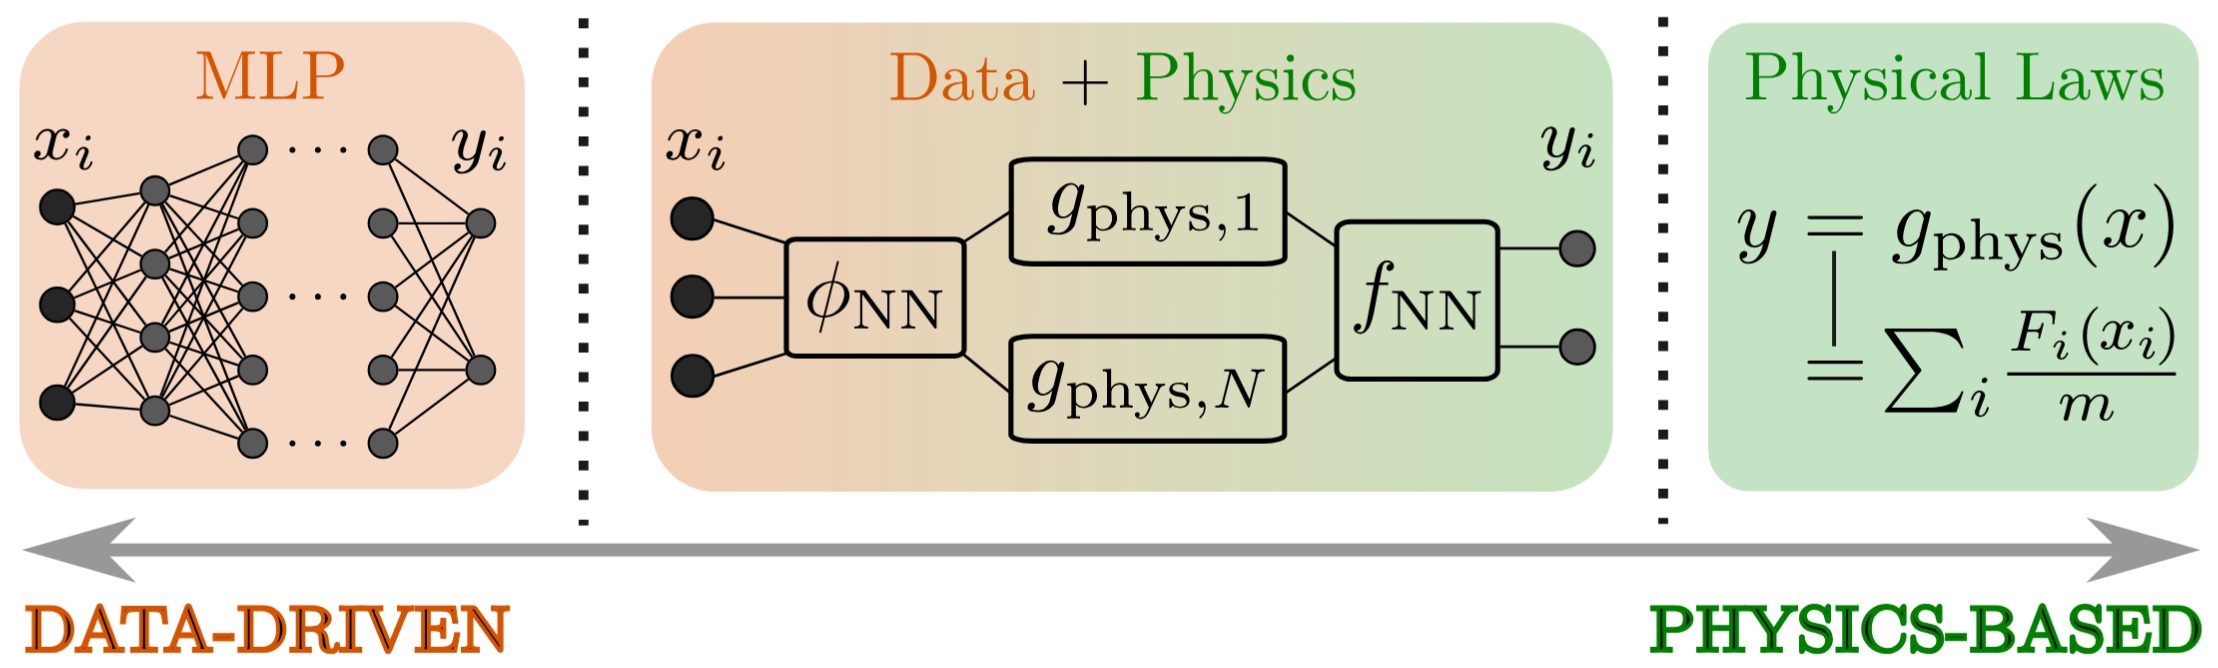
\includegraphics[width=0.85\columnwidth]{figures/diagram_from_model_to_data.pdf}
	\caption{Combining data and physics: In this example, physics-based knowledge is embedded in the architecture of neural networks to model a robot's dynamics, going beyond black-box multi-layer perceptrons (MLPs).}
	\label{fig_curvil_coords_3D}
\end{figure}

\section{General Information} \label{sec_info}
%
\noindent \textbf{Title}: Data Meets Physics: Combining Data-Driven and Physics-Based Approaches in Robotics.\\
%
\textbf{Type}: Half-day workshop.\\
%
\textbf{Organizers}:
%
\begin{enumerate}
	\item Dr. Mattia Piccinini (Primary Contact), Postdoctoral Researcher, Professorship of Autonomous Vehicle Systems, Technical University of Munich, 85748 Garching, Germany. email: mattia.piccinini@tum.de, website: \href{https://www.mos.ed.tum.de/en/avs/team/mattia-piccinini/}{https://www.mos.ed.tum.de/en/avs/team/mattia-piccinini/}.
	\item M.Sc. Baha Zarrouki, Doctoral Researcher, Professorship of Autonomous Vehicle Systems, Technical University of Munich, 85748 Garching, Germany. email: baha.zarrouki@tum.de, website:\\\href{https://www.mos.ed.tum.de/en/avs/team/prof-dr-ing-johannes-betz-2/}{https://www.mos.ed.tum.de/en/avs/team/prof-dr-ing-johannes-betz-2/}.
    \item M.Sc. Dingrui Wang, Doctoral Researcher, Professorship of Autonomous Vehicle Systems, Technical University of Munich, 85748 Garching, Germany. email: dingrui.wang@tum.de, website:\\\href{https://www.mos.ed.tum.de/en/avs/team/dingrui-wang/}{https://www.mos.ed.tum.de/en/avs/team/dingrui-wang/}.
	\item Prof. Gastone Pietro Rosati Papini, Associate Professor, Department of Industrial Engineering, University of Trento, 38123 Trento, Italy. email: gastone.rosatipapini@unitn.it, website: \href{https://tonegas.it}{https://tonegas.it}.
	\item Prof. Johannes Betz, Assistant Professor, Professorship of Autonomous Vehicle Systems, Technical University of Munich, 85748 Garching, Germany. Previously \textbf{organized workshops}: ICRA '24, '22, '21, IROS '25, '24, '21. Co-Chair of the \textbf{RAS Technical Committee} on \textit{Autonomous Ground Vehicles and Intelligent Transportation Systems}. email: johannes.betz@tum.de, website: \href{https://www.mos.ed.tum.de/en/avs/team/prof-dr-ing-johannes-betz/}{https://www.mos.ed.tum.de/en/avs/team/\\prof-dr-ing-johannes-betz/}.
\end{enumerate}
%
\textbf{Website}: \revM{LINK.} We will continuously update the webpage to reflect the list of confirmed speakers as well as
include a call for workshop papers with links to the submission site and paper templates.
%
\section{Abstract} \label{sec_abstract}
%
Machine learning is reshaping robotics, enabling new capabilities in modeling, decision-making, perception and control. However, purely data-driven methods often struggle to deliver generalizable performance in safety-critical applications, where limited training data is available. To address this, recent research has been exploring ways to embed physics-based and classical engineering principles into learning architectures, enhancing interpretability, generalization and sample efficiency. This has led to \textit{physics-driven} learning paradigms that merge the strengths of data-driven and model-based approaches. 

The workshop \textit{Data Meets Physics} at ICRA 2026 will bring together researchers from robotics, machine learning, and control to examine the opportunities and challenges of combining physics-based and data-driven methods. Discussions will focus on embedding domain knowledge into learning frameworks, moving beyond black-box models toward hybrid approaches that couple data with physical insight. Through invited talks, a round table, and a poster session, the workshop will foster knowledge exchange among professors, early-career researchers, and practitioners, encouraging collaboration and innovation in this rapidly-evolving field.
% \revM{Short paragraph (200 WORDS MAXIMUM)}
%
\section{Detailed Workshop Description} \label{sec_detailed_event_description}
%
% \revM{Optional: \textbf{From Action to Perception}. The perception is not about passively constructing an internal representation of the world, but rather about actively picking up information of interest to actions. How can differentiable tools help to guide perception by action?}
%
Topics of interest include the following:
%
\begin{enumerate}
\item \textbf{Beyond black-box learning}. How can we fuse physics-based knowledge with data-driven learning to enhance accuracy and generalization?
\item \textbf{Physics-informed, physics-encoded, physics-guided machine learning and neural operators}. How can domain knowledge be injected into training loss functions, model architectures, constraints, or synthetic data generation pipelines?
\item \textbf{Physics-grounded foundation models} for embodied intelligence. Can large-scale models be constrained or guided by physics to ensure safety, trustworthiness, and transferability to embodied systems?
\item \textbf{From correlation to causation: physical reasoning in robotics}. How can physics-driven machine learning approaches discover causal structures and enhance interpretability in decision-making?
\item \textbf{Applications and challenges across robotics domains}. From modeling and state estimation to planning, control, and decision-making: where do hybrid methods already demonstrate value, and what are the remaining open challenges?
\end{enumerate}

%\begin{itemize}
%\item Approaches exploiting physics-based knowledge to enhance data-driven algorithms
%\item Physics-informed, physics-encoded, physics-guided machine learning
%\item Incorporation of physics-based or domain-specific priors in model architectures, loss functions, constraints or training dataset generation in machine learning frameworks
%\item Foundation models with physics-based grounding or safety assurances
%\item Physical reasoning and causal inference in machine learning
%\item Applications including modeling, control, estimation, planning and decision-making in any field of robotics
%\end{itemize}

%
\section{Structure of the Workshop} \label{sec_structure_of_the_workshop}
%
\begin{table}[h!]
	% \small
	\centering
	\begin{tabular}{c|c|c}
		\toprule 
    \textbf{Time} & \textbf{Event} & \textbf{Notes} \\ 
    \cline{1-3}
    08:30 - 08:35 & Opening & Welcome introduction (5 min) \\
		08:35 - 09:00 & Invited Talk 1 & 20 min + 5 min Q\&A \\
		09:00 - 09:25 & Invited Talk 2 & 20 min + 5 min Q\&A \\
		09:25 - 09:50 & Invited Talk 3 & 20 min + 5 min Q\&A \\
		09:50 - 10:10 & Poster Spotlight & 20 min: 1 min per poster \\
		10:10 - 10:40 & Posters \& Break & 30 min: Poster session + coffee \\ 
		10:40 - 11:05 & Invited Talk 4 & 20 min + 5 min Q\&A \\
		11:05 - 11:30 & Invited Talk 5 & 20
		min + 5 min Q\&A \\
		11:30 - 11:55 & Invited Talk 6 & 20 min + 5 min Q\&A \\
		11:55 - 12:25 & Round Table & 30 min: Panel discussion \\
		12:25 - 12:30 & Closing & Best poster award \& farewell\\
		\toprule
	\end{tabular}
	\caption{Workshop structure.}
	\label{tab_workshop_structure}
  % \vspace{-0.5cm}
\end{table}
%
\subsection{List of Invited Speakers} \label{sec_list_of_invited_speakers}
%
Table \ref{tab_speakers} lists the invited speakers who have confirmed their participation, with their confirmation emails provided in Sec. \ref{sec_appendix}. The speakers represent a wide range of career stages, from post-docs to full professors, as well as diverse genders, geographical origins, and affiliations. Their research covers multiple areas of robotics, including humanoids, soft robotics, autonomous vehicles, and foundation models, all with a strong focus on integrating physics-based and data-driven methods.
%
\begin{table}[h!]
	\centering
	\begin{tabular}{c|c|c|c|c}
		\toprule 
    \textbf{Name} & \textbf{Gender} & \textbf{Position} & \textbf{Affiliation} & \textbf{Country}\\
    \hline
		Ken Goldberg & Male & Full Prof. & UC Berkeley & USA\\
		\hline
		Rolf Findeisen & Male & Full Prof. & TU Darmstadt & Germany\\
		\hline
        Cosimo Della Santina & Male & Associate Prof. & TU Delft & Netherlands\\
		\hline
		Madhur Behl & Male & Associate Prof. & University of Virginia & USA\\
		\hline
		Thomas Beckers & Male & Assistant Prof. & Vanderbilt University & USA\\
		\hline
        Ines Sorrentino & Female & Post-doc & Istituto Italiano di Tecnologia (IIT) & Italy\\
        % Alice Plebe & Female & Post-doc & UCL London & England\\
		\toprule
	\end{tabular}
	\caption{Confirmed speakers.}
	\label{tab_speakers}
\end{table}
%
\section{Plan to Solicit Participation}
%
We plan to solicit participation through multiple channels. Prof. Johannes Betz will promote the workshop within the \textbf{RAS TC} on \textit{Autonomous Ground Vehicles and Intelligent Transportation Systems}, where he serves as Co-Chair. We will also leverage our \textbf{direct connections} with various \textbf{autonomous racing competitions}, where the combination of physics-based and data-driven methods is actively pursued, including \textbf{F1TENTH} Autonomous Racing (80+ partner universities) and the \textbf{Indy Autonomous Challenge} (30+ teams). We will further engage \textbf{industry} collaborators including Honda Research Institute and Bosch, with which we are collaborating on physics-informed machine learning for robotic vehicles. Prof. Papini will promote the workshop within the \textbf{network} of awardees of the Italian \textbf{FIS-2 Starting Grant}, to reach \textbf{early-career PIs} in robotics.

To reach a broader public, we will leverage social media (\textbf{LinkedIn} accounts of the organizers and the TUM-AVS lab, with \textbf{20k+ followers}), our own F1TENTH \textbf{Slack channels} (500+ members), and robotics \textbf{mailing lists} including robotics-worldwide, euRobotics, and the Italian and German robotics communities (ml@automatica.it and rig-all@lists.lrz.de), which we are part of. 
%
% \revM{Please describe (500 WORDS MAXIMUM) how you plan to solicit participation in your event if it is accepted. How do you plan to attract researchers with relevant expertise to attend the event? Steps that go beyond an email to robotics-worldwide are encouraged. If you have organized similar events in the past, estimate the number of participants that you expect. List the titles, organizers, and URLs of the previous events.}
%
\section{Plan to Encourage Interaction}
%
\revM{Describe (500 WORDS MAXIMUM) what steps you will take to encourage interaction among participants. Workshops promote informal discussion of an active research area. How do you plan to promote active discussion between established experts and early-career researchers beyond invited talks and a poster session? Workshop or tutorial proposals that have the potential to increase the number and diversity of participants, encourage participants to stay for the full duration of the event, and promote interaction will be given preference.}
%
\section{Dissemination Plan}
%
\revM{Describe (500 WORDS MAXIMUM) a dissemination plan for the tutorial materials or the contributed papers, contributed talks, and outcomes of the workshop. Creating an accessible online archive for media, articles, and discussions is strongly encouraged. Please describe the process and how access will be provided to participants and ICRA 2026 attendees. Strategies for reaching a broad audience, including researchers from traditionally underrepresented backgrounds, will be viewed as a particular strength. Workshop papers should encourage and prioritize the submission of new ideas. A workshop paper submission may be a non-archival abstract based on a prior publication. However, it cannot take the form of an existing paper that is published or under review, and it cannot be considered published as a peer-reviewed paper.}
%
\section{Additional Information}
%
\subsection{Improving Diversity and Inclusion}
%
\revM{Describe (500 WORDS MAXIMUM) the steps you will take to enhance diversity and inclusion among participants. Outline your plans to ensure diverse and inclusive participation and interaction beyond invited talks and poster sessions. Proposals that show strong potential to increase participant diversity, promote inclusive engagement throughout the event, and foster meaningful interactions among a varied group of attendees will be given preference.
}
%
\subsection{Compliance with RAS Guidelines and Code of Conduct}
%
We confirm that the organizers will be present in person at the workshop and will ensure that the workshop fully complies with the RAS Guidelines.

We confirm that we have read the IEEE RAS Code of Conduct and agree to abide by it. We shall also inform the speakers and all the workshop participants about the code of conduct by either communicating it directly to them or by including a link to it on our workshop website.
%
\subsection{Previous Workshop Organization Experience}
%
\section{Appendix: Emails from Invited Speakers} \label{sec_appendix}
%
\end{document}